\chapter{Tecnologías empleadas}
\label{cap:tecnologiasEmpleadas}
En este capítulo se explican todas la tecnologías, aplicaciones y herramientas que se han utilizado durante el proceso de desarrollo. El capítulo se ha dividido en dos apartados principales, uno dedicado a tecnologías generales y otro dedicado a tecnologías específicas del desarollo Android.

\section{Aplicaciones y herramientas generales}
\hypertarget{subsec:android_studio}{}
\subsection{Android Studio}
\href{https://developer.android.com/studio/intro}{Android Studio} es el entorno de desarrollo integrado (IDE) oficial utilizado para el desarrollo de aplicaciones en Android. Esta basado en \href{https://www.jetbrains.com/idea}{Intellij Idea}, un editor multiplataforma con soporte para lenguajes como \hyperlink{subsec:kotlin}{Kotlin}, \href{https://www.java.com}{Java} y \href{https://www.scala-lang.org}{Scala} entre otros. 

Android Studio ha sido utilizado a lo largo del proceso completo de desarrollo, siendo de gran utilidad sus modernas funcionalidades como ayuda al correcto flujo de trabajo. Este entorno te permite utilizar emuladores para probar las aplicaciones, sin embargo estos emuladores consumen gran cantidad de recursos del ordenador, esto ha sido un poco problemático en el caso de este proyecto ya que el ordenador con el que se contaba para el desarrollo no contaba con recursos suficientes para ejecutar el emulador correctamente, provocando en algunos casos problemas de \textit{lag} y \textit{crashes} ocasionales. A pesar de esto, ha sido posible desarrollar la aplicación usando estos emuladores.

\subsection{Obsidian}
\href{https://obsidian.md/}{Obsidian} es una aplicación de código abierto que sirve como sistema de notas, te permite organizar las mismas con gran cantidad de posibilidades. Cuenta con funcionalidades que han sido de gran utilidad como la referenciación entre notas, vista de grafo y multitud de extensiones desarrolladas por la comunidad.

En este proyecto, Obsidian ha servido como complemento al desarrollo. Se ha utilizado, entre otras cosas, para la planificación de hitos (apuntes personales sobre los casos de uso, fechas de entrega, dudas para tutoría...), reunión de ideas sobre las funcionalidades y documentación del ciclo de vida del proyecto.

\hypertarget{subsec:figma}{}
\subsection{Figma}
\href{https://www.figma.com}{Figma} es una plataforma de diseño basada en la web que permite crear y prototipar diseños de interfaces de usuario, con ella ha sido posible crear diseños de una forma rápida y eficaz, que luego han sido materializados en \hyperlink{subsec:compose}{Jetpack Compose}. 

En este proyecto en particular, figma ha sido utilizada para plasmar las ideas de diseño, sirviendo estas como una referencia no estricta de las interfaces finales. En el apéndice \ref{Appendix:interfacesfigma} se han adjuntado capturas de pantalla de todas las interfaces diseñadas. Como la aplicación se ha desarrollado utilizando \href{https://m3.material.io/}{Material 3} y \href{https://m3.material.io/styles/color/system/overview}{Dynamic Colors} (véase la subseccion \ref{subsec:material_design} para más detalles acerca de Material design) los colores varían dinámicamente en función del tema de cada dispositivo por lo que los colores de los diseños de figma no tienen por qué corresponderse con los colores que luego se han materializado en cada dispositivo.
\hypertarget{subsec:drawio}{}
\subsection{Drawio}
\href{https://www.drawio.com/}{Drawio} es una herramienta de código abierto que permite a los usuarios crear una amplia variedad de diagramas (flujo, Gantt...), seleccionada para el proyecto por ser cómoda, personalizable y con gran capacidad de portabilidad, utilizando ficheros con extensión .io y dando la capacidad al usuario de cambiar de herramienta con facilidad. 

Esta aplicación ha sido utilizada para la realización de todos los diagramas que han sido necesarios durante el proyecto. Ha sido especialmente útil para el diseño de las bases de datos del proyecto (véase el apéndice \ref{Appendix:bd_design} con los diseños) ya que, al haberse utilizado bases de datos no SQL, ha sido necesario depurar el diseño en varias ocasiones para evitar la duplicación lo máximo posible.

\subsection{Git, Github y Lazygit}
Para el control de versiones de la aplicación se ha utilizado la conocida herramienta utilizada por la gran mayoría de los desarrolladores de software a nivel mundial: \href{https://git-scm.com/}{Git}. Pese a haber sido un proyecto desarrollado por una sola persona, Git ha sido una herramienta esencial para el proceso de desarrollo, sirviendo como backup en el desarrollo de nuevas funcionalidades y como control general del estado de la aplicación. 

El repositorio con el código de la aplicación y el código latex utilizado para la redacción de esta memoria se han almacenado de forma pública en \href{https://github.com/}{Github}, plataforma de desarrollo colaborativo basada en la web que utiliza Git como sistema de control de versiones.

También merece mención en este apartado la herramienta de código abierto \href{https://github.com/jesseduffield/lazygit}{Lazygit}, interfaz gráfico de terminal para linux que proporciona una forma fácil y visual de interactuar con los repositorios Git. Está diseñado para simplificar el flujo de trabajo al proporcionar una interfaz gráfica intuitiva dentro de la terminal. Ha sido de gran ayuda para la agilización del uso de Git a lo largo del desarrollo del proyecto en conjunción con la extension de \hyperlink{subsec:android_studio}{Android Studio} para Git.
\section{Tecnologías específicas de Android}

\hypertarget{subsec:kotlin}{}
\subsection{Kotlin}
\href{https://kotlinlang.org/}{Kotlin} es un lenguaje de programación de código abierto creado por JetBrains, es un lenguaje de tipado estático, lo que significa que se puede desarrollar sobre la JVM (Java Virtual Machine) y es totalmente compatible e interoperable con Java lo que facilita la migración desde el primero \footnote{Artículo que explica en detalle qué es kotlin: \href{https://www.plainconcepts.com/es/kotlin-android/}{Plain Concepts}}. 

Este lenguaje de programación ha sido seleccionado para el proyecto ya que, a parte de ser el recomendado por Google y ser muy cómodo y útil de usar, con el paso de los años se está consolidando como el lenguaje de referencia para el desarrollo Android, dejando obsoleto el anterior lenguaje de referencia: Java.
\subsubsection{Kotlin vs. Java}
\label{subsec:kotlinvsjava}
Kotlin empezó a considerarse como una opción viable para el desarrollo Android en 2017, cuando Google le empezó a dar soporte. En ese momento, Java era el lenguaje universal utilizado para el desarrollo de aplicaciones en Android. A partir de este punto, en los siguientes años comenzó el debate de si Kotlin era mejor alternativa. En estos últimos años este debate ha quedado prácticamente resuelto en favor de Kotlin, que ha demostrado ser un lenguaje mucho más moderno y útil dejando obsoleto a Java.

Algunas de las características -entre muchas otras- que hacen a kotlin destacar por encima de java son:
\begin{itemize}
    \item Una sintaxis más moderna más moderna, que permite hacer más con menos código.
    \item Al ser el lenguaje principal utilizado para Android hoy en día ofrece un mayor -y más actualizado- número de bibliotecas, más comunidad y recursos diponibles.
    \item Inmutabilidad de variables: una variable no puede cambiar a no ser que se indique explicitamente que sí. Esto ahorra mucho posibles errores.
    \item Kotlin está diseñado ser un lenguaje \textit{null-safe}, es decir ofrece seguridad sobre valores nulos (¡No más NullPointerException!). Esto quiere decir que los valores no pueden ser nulos por defecto, para serlo se debe indicar expresamente con el operador ‘?’.
    \item Relativo a Android, ofrece soporte nativo para corrutinas y flows, muy útiles en el desarrollo de aplicaciones.
\end{itemize}
A continuación se muestra una breve comparación del mismo código -que declara una variable, sumándola a un número entero, guardándola en otra variable y mostrándola por consola- en los dos lenguajes para intentar ilustrar algunas de las diferencias entre ambos:
\begin{figure}[h]
	\centering
	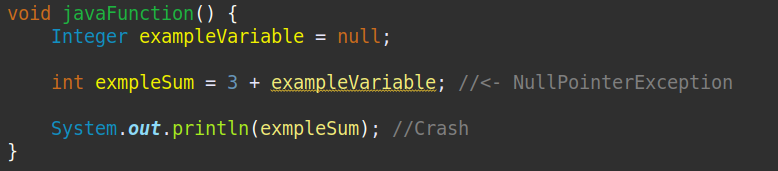
\includegraphics[width = 1\textwidth]{Imagenes/Fuentes/javaFun.png}
	\caption{Función en Java}
	\label{fig:javaFun}
\end{figure}
\begin{figure}[h]
	\centering
	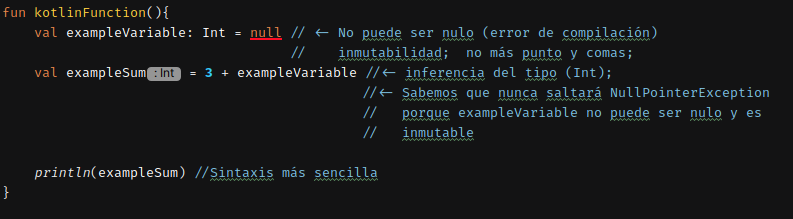
\includegraphics[width = 1\textwidth]{Imagenes/Fuentes/kotlinFun.png}
	\caption{Función en Kotlin}
	\label{fig:kotlinFun}
\end{figure}

\hypertarget{subsec:compose}{}
\subsection{Jetpack Compose}
\href{https://developer.android.com/develop/ui/compose}{Jetpack Compose} es un moderno kit de herramientas de desarrollo de interfaces de usuario (UI) para Android, desarrollado por Google. Permite a los desarrolladores construir interfaces de usuario de aplicaciones de forma más fácil y eficiente, utilizando un enfoque declarativo. Jetpack Compose fue elegida como tecnología principal para el desarrollo de las interfaces porque suponía un reto apasionante, es una tecnología puntera y muy demandada actualmente en el mundo profesional. Por estos motivos, desde el principio del desarrollo de Profinder se decidió utilizar. 

Jetpack Composes es una forma más cómoda, sencilla y mejor de desarrollar aplicaciones frente al sistema tradicional de vistas con XML. A continuación se intenta explicar el por qué de esta afirmación.
\subsubsection{Jetpack Compose vs. Android views}
Android Views son el enfoque tradicional para construir interfaces de usuario en aplicaciones Android. Se definen principalmente utilizando archivos XML y se gestionan programáticamente en Java o Kotlin. Esta era la forma de desarrollar interfaces en Android hasta que a partir de 2019, cuando salió Jetpack Compose en modo \textit{preview}, ambas fueron poniendose a la par. Fue en 2021 cuando Google estableció Jetpack Compose como la forma recomendada de aprender a desarrollar aplicaciones en Android. Hoy en día, Jetpack Compose está totalmente asentado y es un hecho que cada vez va dejando más atrás el sistema de vistas y es algo lógico puesto qeu presenta numerosas ventajas:
\begin{itemize}
    \item Todo en Kotlin: mientras que usando Views las interfaces se definen en XML y se manipulan programáticamente en kotlin -o Java, pero no lo tendremos en cuenta para esta comparativa debido a que ya ha sido realizada en la seccion \ref*{subsec:kotlinvsjava}- en Jetpack Compose se unifica todo en kotlin. Esto reduce enormemente la cantidad de código necesaria y hace el código mucho más entendible
    \item Jetpack Compose ofrece un estilo de programación declarativa y reactiva que se adapta mucho mejor al paradigma de programación funcional de Kotlin, apoyándose mucho por ejemplo, en el uso de \href{https://kotlinlang.org/docs/lambdas.html}{lambdas} para añadir robustez al código.
    \item Debido a que Jetpack Compose es hoy en día la principal forma de programar interfaces, constanmente van saliendo actualizaciones y nuevas utilidades como el \textit{live edit}, que permite ver los cambios en diseño de tu aplicación en tiempo real mientras que esta está ejecutandose; o las \textit{previews} que permiten comprobar el diseño en distintos dispositivos y tamaños.
    \item Jetpack Compose permite programar para distintos tipos de dispositivos, esto significa que se podría por ejemplo, crear en el mismo proyecto una aplición de móvil su versión de wearable y su versión de escritorio sin más complicación que la que tuviero adaptar las interfaces a cada tamaño.
\end{itemize}
Para terminar esta comparativa, a continuación se muestran dos formas de hacer exactamente lo mismo (una columna que renderice y muestre los elementos en pantalla) utilizando las dos formas analizadas en este apartado. Como se puede comprobar lo que se hace en 6 líneas de código en Jetpack Compose necesita de tres clases en el sistema de vistas (Adapter, Viewholder y Activity):
\begin{figure}[h]
	\centering
	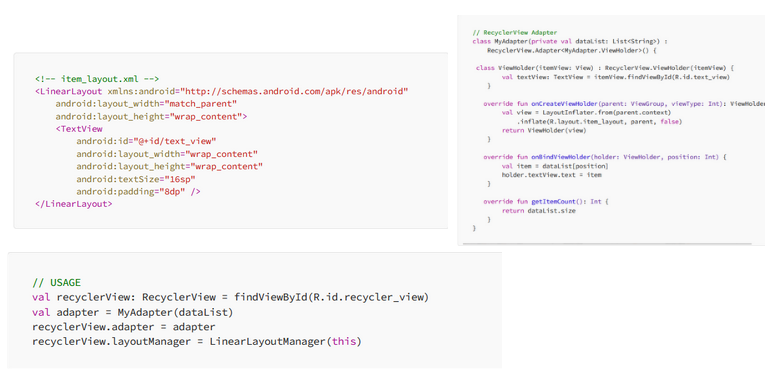
\includegraphics[width = 1\textwidth]{Imagenes/Fuentes/views_demo.png}
	\caption{Recycler View utilizando Android views \citep{RecyclerVsLazy}}
	\label{fig:views_demo}
\end{figure}
\newpage
\begin{figure}[h]
	\centering
	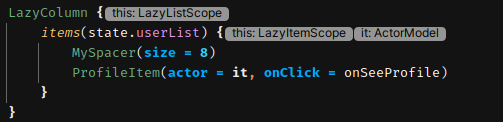
\includegraphics[width = 1\textwidth]{Imagenes/Fuentes/compose_demo.png}
	\caption{LazyColumn utilizando Jetpack Compose}
	\label{fig:compose_demo}
\end{figure}

\subsection{Testing}
\label{subsec:testing}
Durante el proceso de desarrollo de Profinder, se han encontrado numerosos desafíos que resolver pero sin duda el testing ha sido el más complicado. La cantidad de cosas que se pueden hacer y conocimientos que aprender son un mundo y debido a los ajustados tiempos del proyecto solo ha sido posible rascar la superficie.

Se han implementado pequeños test unitarios usando librerías como \href{https://mockk.io/ANDROID.html}{mockk} sobretodo del repositorio, en el que se han podido probar todas las funciones. También se han podido probar algunos casos de uso y se ha intentado probar los viewmodel, pero debido a la complejidad sus pruebas no ha dado tiempo ha hacer algo que de verdad valga la pena, por eso los tests se clasificarán en el capítulo \ref{cap:conclusiones} como una línea de trabajo futuro.

\subsection{Dagger Hilt}
Todo el proyecto ha sido implementado utilizando inyección de dependencias mediante \href{https://dagger.dev/hilt/}{Dagger Hilt}. 

Dagger Hilt es un framework que realiza operaciones en tiempo de compilación (autogenerando ficheros) para Android, el cual se encarga de crear y administrar la creación de objetos en toda la aplicación, esto tiene muchas ventajas pero la principal es que facilita la codificación inmensamente ya que evita tener que saber donde se crea cada objeto.
\begin{figure}[h]
	\centering
	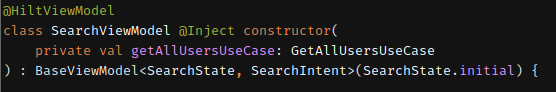
\includegraphics[width = 1\textwidth]{Imagenes/Fuentes/ejemplo_hilt1.png}
	\caption{Ejemplo de inyección de un caso de uso usando Hilt}
	\label{fig:ejemplo_hilt1}
\end{figure}

Se han creado módulos para inyectar todos los servicios remotos de \hyperlink{subsec:firebase}{Firebase}, así como para el servicio de localización, creando automáticamente instancias que serán utilizadas por todas las interfaces que las requieran.
\newpage
\begin{figure}[h]
	\centering
	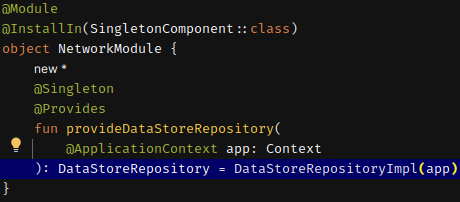
\includegraphics[width = 0.7\textwidth]{Imagenes/Fuentes/ejemplo_hilt2.png}
	\caption{Ejemplo de módulo de dependencias}
	\label{fig:ejemplo_hilt2}
\end{figure}

Por último, en todas las vistas se han inyectado los \textit{viewmodels}:
\begin{figure}[h]
	\centering
	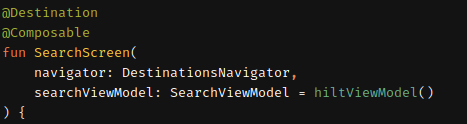
\includegraphics[width = 0.7\textwidth]{Imagenes/Fuentes/ejemplo_hilt3.png}
	\caption{Ejemplo de viewmodel inyectado}
	\label{fig:ejemplo_hilt3}
\end{figure}

\subsection{Maps}
Para el desarrollo de la funcionalidad del mapa, ha sido necesario utilizar el \href{https://developers.google.com/maps/documentation/android-sdk}{SDK de Google Maps para Android}. Para utilizarlo es necesario darse de alta en la consola de Google para desarrolladores e introducir un método de pago (aunque el límite de uso gratuito es bastante por lo que esto no supone un problema) para recibir la clave de API necesaria.

Una vez obtenida la clave de API ya es posible implementar mapas en la aplicación, para ello se utilizó una adaptación del SDK para el uso en \hyperlink{subsec:compose}{Jetpack Compsose} creada por múltiples desarrolladores de Google como herramienta \textit{open source}.
\footnote{Link al repositorio: \href{https://github.com/googlemaps/android-maps-compose}{android-maps-compose}}
\begin{figure}[h]
	\centering
	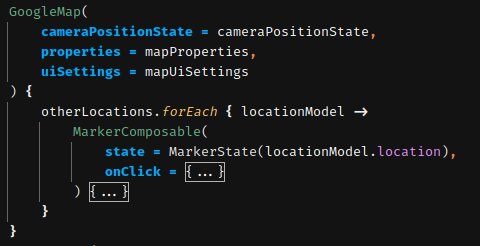
\includegraphics[width = 0.6\textwidth]{Imagenes/Fuentes/maps_compose.png}
	\caption{Uso del \textit{composable} GoogleMap para dibujar un mapa en la aplicación}
	\label{fig:maps_compose}
\end{figure}
\subsection{Compose Destinations}
La navegación nativa que ofrece \hyperlink{subsec:compose}{Jetpack Compsose} no es demasiado cómoda por el momento ya que usa navegación por rutas en formato de \textit{string}, lo cual puede llegar a ser confuso y poco seguro. 

Para solucionar este problema se ha encontrado una biblioteca creada por la comunidad llamada \href{https://github.com/raamcosta/compose-destinations}{Compose Destinations}. Esta biblioteca utiliza como base la navegación nativa pero añade una capa encima que permite estructuración y tipado de los argumentos, ofreciendo una navegación más segura y sencilla de utilizar. Este recurso ha sido muy útil, haciendo el desarrollo con múltiples vistas sustancialmente más sencillo.

Para utilizarlo solo hay que utilizar el tag \textit{Destination} en la funciones que participen en la navegación, esta etiqueta autogenera el código necesario -usando la navegación nativa- en tiempo de compilación. 
\begin{figure}[h]
	\centering
	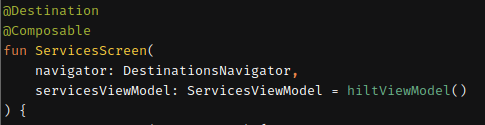
\includegraphics[width = 0.6\textwidth]{Imagenes/Fuentes/ejemplo_destination.png}
	\caption{Ejemplo de declaración de función como Destination.}
	\label{fig:ejemplo_destination}
\end{figure}

Una vez generado este código se podrá utilizar la variable \textit{navigator} para navegar a esas pantallas de forma sencilla. 
\begin{figure}[h]
	\centering
	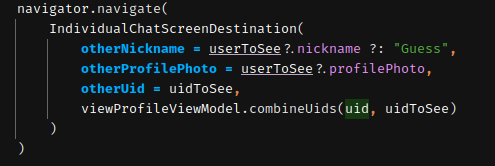
\includegraphics[width = 0.6\textwidth]{Imagenes/Fuentes/ejemplo_navigator.png}
	\caption{Ejemplo de uso de variable navigator.}
	\label{fig:ejemplo_navigator}
\end{figure}

\hypertarget{subsec:coil}{}
\subsection{Coil} 
\href{https://coil-kt.github.io/coil/compose/}{Coil} es una biblioteca creada para \hyperlink{subsec:compose}{Jetpack compose} (equivalente a \href{https://github.com/bumptech/glide}{Glide} en Android views). Sirve para cargar imágenes en las interfaces, proporciona el componente AsyncImage que se ha utilizado para mostrar las fotos de perfil de los usuarios en la aplicación. Se ha optado por Coil en lugar de bibliotecas como \href{https://square.github.io/picasso/}{Picasso} ya que ofrece un rendimiento e integración con \hyperlink{subsec:compose}{Jetpack compose} mucho mejor. 
\subsection{Material design}
\label{subsec:material_design}
\href{https://m3.material.io/}{Material Design} es un sistema de diseño creado por Google que se utiliza para crear experiencias de usuario coherentes y atractivas en aplicaciones. 

Para esta aplicación se ha utilizado Material 3 que ofrece la funcionalidad de Dynamic colors, esto significa que no tiene una paleta de colores estática, sino que dependiendo del tema de cada dispositivo específico, crea una paleta de colores personalizada. De esta forma se consigue una mejor experiencia de usuario, que gracias al algoritmo que se usa para crear la paleta de colores mantiene la armonía entre aplicaciones que usen Material.

Gracias a este sistema, también ha sido posible hacer la aplicación con tema claro y oscuro, para conseguir esto se declaran dos colores para cada elemento de la paleta de colores (dinámicamente) y en función de una variable \textit{booleana} controlada por la aplicación se decide que tema se utiliza.